%\documentclass[12pt]{article}
%\usepackage[margin=1in]{geometry} 
%\usepackage{amsmath,amsthm,amssymb,amsfonts}
%\usepackage{graphicx}
%\usepackage{float} 
%\newcommand{\N}{\mathbb{N}}
%\newcommand{\Z}{\mathbb{Z}}
%\newenvironment{problem}[2][Problem]{\begin{trivlist}
%		\item[\hskip \labelsep {\bfseries #1}\hskip \labelsep {\bfseries #2.}]}{\end{trivlist}}
%\begin{document}

\begin{figure}[h]
\centering
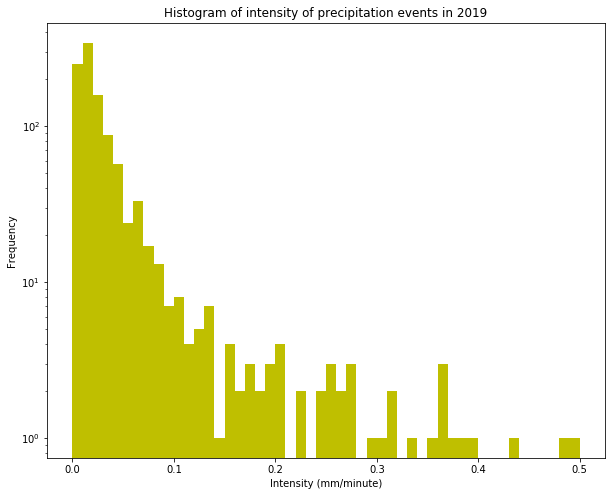
\includegraphics[width=0.5\textwidth]{../Figures/intensity_hist_5min.png}
\caption{\label{abc}Distribution of intensity of precipitation events
  in 2019, defined as the total precipitation divided by the
  duration. This distribution was derived from the distribution of
  duration of precipitation with a minimum duration of 5 minutes. The
  distribution decreases logarithmically from 0.01 mm/minute to 0.5
  mm/minute.}
\end{figure}
\vfill
\begin{figure}[h]
\centering
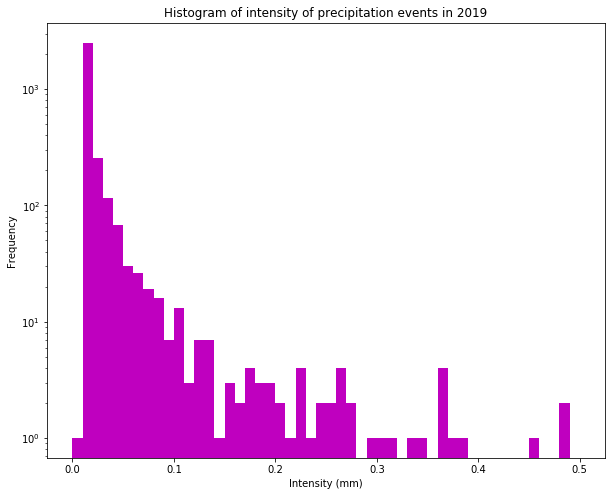
\includegraphics[width=0.5\textwidth]{../Figures/intensity_hist_1min.png}
\caption{\label{abcd}Distribution of intensity of precipitation events
  in 2019, defined as the total precipitation divided by the
  duration. This distribution was derived from the distribution of
  duration of precipitation with a minimum duration of 1 minute. The
  distribution decreases logarithmically from 0.01 mm/minute to 0.5
  mm/minute.}
\end{figure}
\vfill
\begin{figure}[h]
\centering
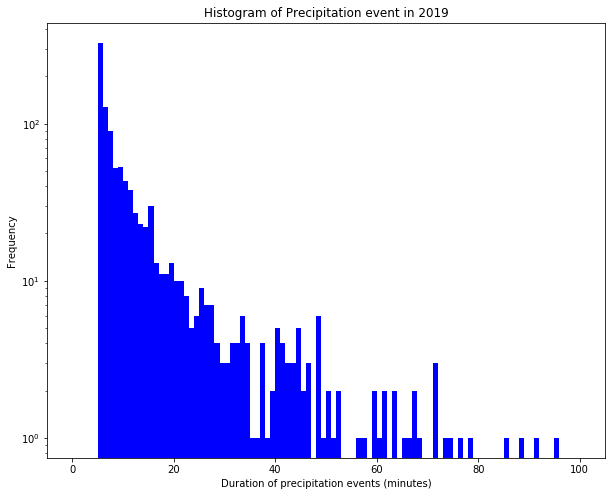
\includegraphics[width=0.5\textwidth]{../Figures/precip_hist_5min.png} 
\caption{\label{abce}Distribution of duration of precipitation events
  in 2019. 5 minutes was the minimum duration needed to define a
  precipitation event. The distribution is decreasing logarithmically
  from the highest values in the 5 minute precipitation events and the
  lowest values approaching 100 minutes.}
\end{figure}
\begin{figure}[h]
\centering
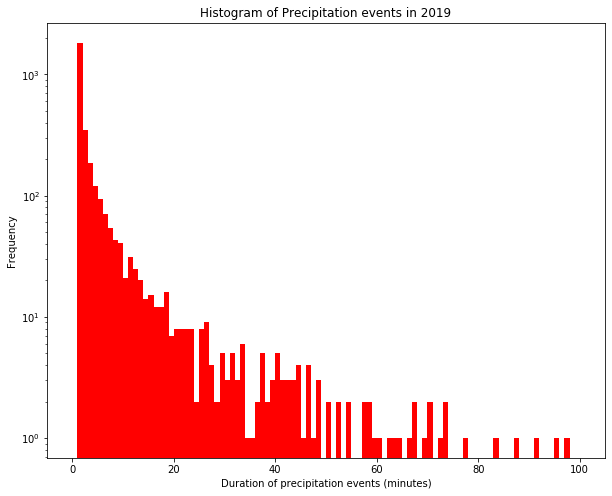
\includegraphics[width=0.5\textwidth]{../Figures/precip_hist_1min.png}
\caption{\label{abcf}A histogram that shows the duration of
  precipitation event. Note that in this histogram that the 1 minute
  was the minimum duration needed to define a precipitation event. As
  expected, the distribution is that we have most precipitation events
  be close to the minimum duration and that less precipitation events
  are particularly long. }
\end{figure}
\begin{figure}[h]
\centering 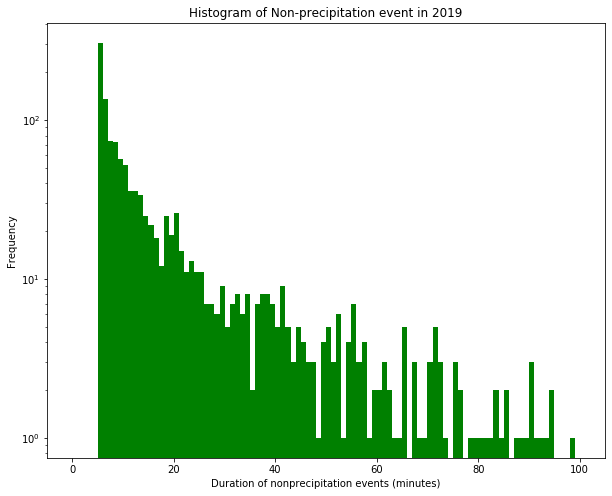
\includegraphics[width=0.5\textwidth]{../Figures/nonprecip_hist_5min.png} 
\caption{\label{abcg}This is a histogram for the duration of a
  non-precipitation event, which is to say the gap between two
  precipitation events. It also follows the pattern of having lots of
  the non-precipitation events be close to the minimum
  non-precipitation event of 5 minutes. It does look like that there
  are more non-precipitation events that lasts longer than say 40
  minutes compared to the precipitation events. }
\end{figure}
\begin{figure}[h]
\centering
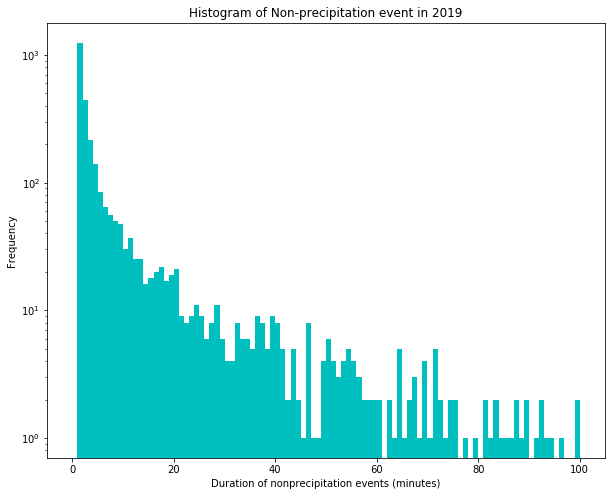
\includegraphics[width=0.5\textwidth]{../Figures/nonprecip_hist_1min.png}
\caption{\label{abch}This is a histogram for the duration of a
  non-precipitation event, which is to say the gap between two
  precipitation events. Most events do seem to lie close to the
  minimum duration of 1 minute.}
\end{figure}
\begin{figure}[h]
\centering 
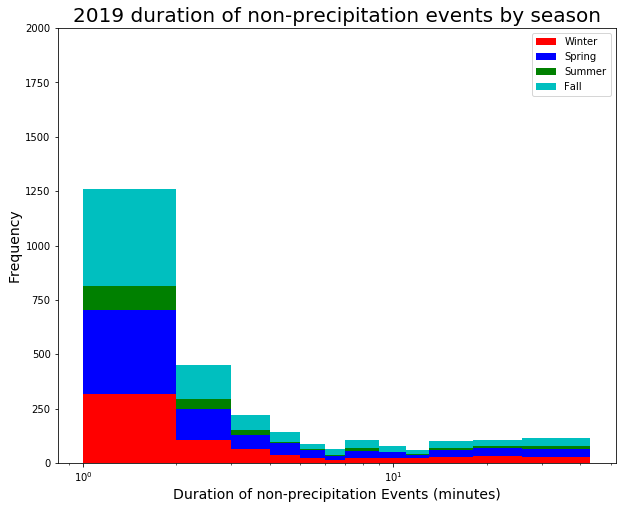
\includegraphics[width=0.5\textwidth]{../Figures/nonprecip1mm_season_19.png} 
\caption{\label{abci}Distribution of the duration of non-precipitation
  events separated by seasons. The distribution within each season
  does indeed decrease exponentially as we go from 1 minute duration
  to about 40 minute duration, with the extreme 98th to 100th
  percentile excluded.}
\end{figure}
\begin{figure}[h]
\centering
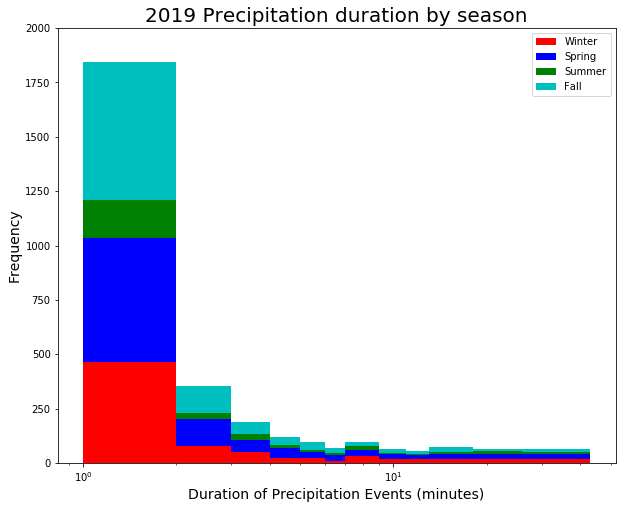
\includegraphics[width=0.5\textwidth]{../Figures/precip1mm_season_19.png}
\caption{\label{abcj}Distribution of the duration of precipitation
  events separated by seasons. The distribution for each season does
  decrease exponentially from 1 minute to 40 minute durations. It does
  seem like the more precipitation events are closer to the minimum
  precipitation duration compared to the non-precipitation events.}
\end{figure}
\begin{figure}[h]
\centering 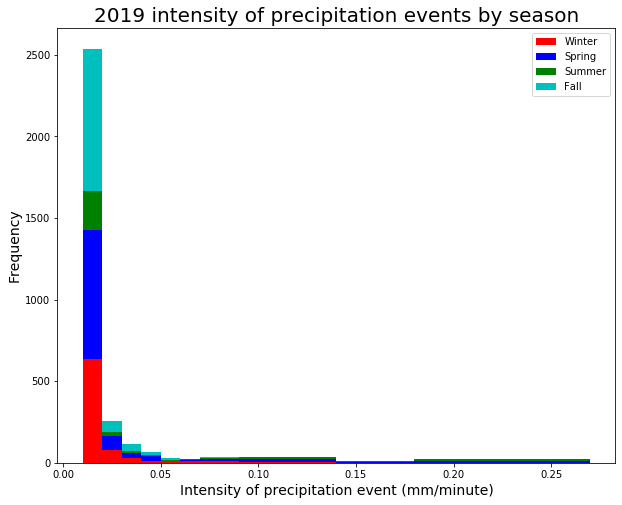
\includegraphics[width=0.5\textwidth]{../Figures/inten1mm_season_19.png} 
\caption{\label{abck}Distribution of intensity of precipitation events
  separated by seasons. The distribution decrease for each season from
  0.01 mm/minute to 0.27 mm/day.}
\end{figure}
\begin{figure}[h]
\centering
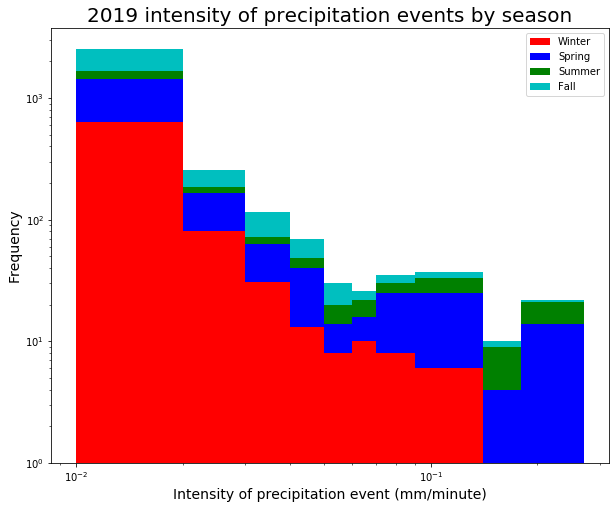
\includegraphics[width=0.5\textwidth]{../Figures/inten1mm_season_19_log.png}
\caption{\label{abcl}Shows the previous figure in terms of log scale
  for both x and y axis. It shows that winter does not have very
  intense precipitation events and that despite Summer and Winter
  having similar amounts of precipitation, (232 mm for Summer to 240
  mm for Winter), summer seems to have more intense precipitation
  events.}
\end{figure}
%\end{document}
